\documentclass[conference]{IEEEtran}

\usepackage[T1]{fontenc}
\usepackage[utf8]{inputenc}
\usepackage{amsmath,amssymb}
\usepackage{graphicx}
\usepackage{booktabs}
\usepackage{multirow}
\usepackage{xcolor}
\usepackage{hyperref}
\usepackage{cite}
\usepackage{url}
\usepackage{microtype}
\usepackage{subcaption}

\graphicspath{{figures/}}

\hypersetup{
  colorlinks=true,
  linkcolor=blue!60!black,
  citecolor=blue!60!black,
  urlcolor=blue!60!black
}

% =========================================================
\begin{document}

\title{A Comparative Study of Variational Autoencoder and DnCNN\\
for Image Denoising: Quantitative Evaluation and\\
Computational Analysis}

\author{
  \IEEEauthorblockN{Abdullah Al Mahmud}
  \IEEEauthorblockA{
    Department of Computer Science \& Engineering\\
    BRAC University\\
    Dhaka, Bangladesh\\
    \texttt{abdullah.al.mahmud@g.bracu.ac.bd}
  }
}

\maketitle

% =========================================================
\begin{abstract}
Image denoising is a foundational problem in computer vision with
critical applications in medical imaging, remote sensing, and digital
photography. Deep learning has produced two distinct paradigms for
addressing this challenge: discriminative models that directly learn a
mapping from noisy to clean images, and generative models that learn the
underlying distribution of clean images. This paper presents a rigorous
comparative evaluation of the Denoising Convolutional Neural Network
(DnCNN), a canonical discriminative model, and the Variational
Autoencoder (VAE), a representative generative model, under identical
experimental conditions. Both architectures are trained on the BSD300
dataset and evaluated on the BSD68 benchmark across Gaussian and Poisson
noise at severity levels \(\sigma \in \{15, 25\}\), using Peak
Signal-to-Noise Ratio (PSNR), Structural Similarity Index (SSIM), and
Learned Perceptual Image Patch Similarity (LPIPS) as evaluation metrics.
Results demonstrate that DnCNN consistently outperforms VAE in all
quantitative metrics, achieving up to 11.26 dB higher PSNR on Gaussian
noise at \(\sigma = 25\). DnCNN also exhibits significantly faster
inference, requiring 1.50 ms per image compared to 40.61 ms for the VAE.
These findings suggest that DnCNN is the preferred architecture for
standard denoising pipelines, while the VAE's probabilistic formulation
offers complementary advantages for uncertainty quantification and
cross-noise generalization.
\end{abstract}

\begin{IEEEkeywords}
image denoising, variational autoencoder, DnCNN, convolutional neural
network, PSNR, SSIM, LPIPS, Gaussian noise, Poisson noise, deep learning
\end{IEEEkeywords}

% =========================================================
\section{Introduction}

Digital images are inherently susceptible to noise introduced during
acquisition, transmission, and storage. Noise degrades image quality,
reduces visual clarity, and complicates downstream computer vision tasks
such as object detection, segmentation, and classification. In medical
imaging -- including MRI, CT, and ultrasound -- noise can obscure
clinically relevant features and potentially lead to misdiagnosis. In
remote sensing and surveillance, noise hampers accurate scene
interpretation. Effective image denoising is therefore not merely an
aesthetic concern but a critical preprocessing step in many real-world
pipelines.

Classical approaches such as Non-Local Means (NLM) and BM3D have long
served as benchmarks by exploiting patch-based self-similarity through
mathematically elegant formulations. However, they suffer from two
fundamental limitations: careful hyperparameter tuning is required for
different noise types, and their inference cost is substantial due to
iterative optimization at test time.

The deep learning revolution has produced data-driven denoisers that
learn denoising priors directly from large image collections. Two
paradigms have emerged as particularly influential. \textit{Discriminative
models} directly learn a mapping from noisy to clean images;
\textit{generative models} learn the underlying distribution of clean
images and exploit this prior during denoising. DnCNN \cite{zhang2017beyond}
and the Variational Autoencoder (VAE) \cite{kingma2014vae} are the
canonical representatives of these two paradigms, respectively.

Despite their widespread adoption, a systematic, controlled comparison
under identical experimental conditions is not well established in the
literature. Most published comparisons focus on introducing new
architectures and compare against selected baselines, rather than
examining the fundamental trade-offs between generative and discriminative
denoising frameworks. This paper addresses that gap directly.

\subsection{Contributions}

The specific contributions of this work are as follows:
\begin{itemize}
  \item A clean, reproducible implementation of both DnCNN and VAE for
    grayscale image denoising, released with all training and evaluation
    code.
  \item A quantitative evaluation on the BSD68 benchmark across two
    noise types (Gaussian, Poisson) and two noise levels
    (\(\sigma \in \{15, 25\}\)) using three complementary metrics: PSNR,
    SSIM, and LPIPS.
  \item A computational efficiency analysis covering parameter count and
    inference latency.
  \item Evidence-based observations on the qualitative behaviour of both
    models regarding texture preservation, edge sharpness, and artefact
    generation.
\end{itemize}

% =========================================================
\section{Related Work}

\subsection{Classical Denoising Methods}

The earliest approaches to image denoising relied on explicit
mathematical models of image smoothness. Gaussian and bilateral filtering
suppress noise by averaging pixel values within a neighbourhood weighted
by spatial and intensity proximity. Total Variation (TV) regularization
promotes piecewise-smooth solutions while preserving sharp edges, though
TV-based methods tend to produce characteristic staircase artefacts.

Buades \textit{et al.} proposed Non-Local Means (NLM), which exploits
natural patch redundancy by computing a weighted average over all pixels
whose local neighbourhoods resemble the target pixel. Dabov \textit{et al.}
extended this to BM3D, which groups similar patches and processes them
collaboratively in the transform domain, remaining state-of-the-art for
nearly a decade. Dictionary learning methods such as K-SVD achieved
competitive results but require iterative optimization at test time.

\subsection{Deep Learning-Based Denoising}

Burger \textit{et al.} demonstrated that a plain multi-layer perceptron
trained on image patches could match BM3D performance. Mao \textit{et al.}
introduced RED-Nets, very deep residual encoder-decoder networks with
symmetric skip connections. The U-Net architecture, originally developed
for biomedical segmentation, has been widely adapted for image restoration.

Generative Adversarial Networks have been applied to image restoration
with visually impressive results, though they are prone to training
instability and hallucinated texture. Transformer-based architectures
including Restormer and SwinIR currently define state-of-the-art on most
restoration benchmarks. Diffusion models have also been adapted for image
restoration, achieving high perceptual quality at the cost of slow
inference.

\subsection{Autoencoders and Variational Autoencoders}

Autoencoders learn compressed latent representations through an
encoder-decoder bottleneck. Vincent \textit{et al.} introduced Denoising
Autoencoders (DAEs), explicitly trained to reconstruct clean inputs from
corrupted ones. Kingma and Welling \cite{kingma2014vae} proposed the
Variational Autoencoder, extending this framework with a probabilistic
latent space. Several works have adapted VAEs for denoising in medical
imaging and general image restoration settings.

\subsection{Discriminative CNN Denoisers}

Zhang \textit{et al.} \cite{zhang2017beyond} proposed DnCNN, which
predicts the noise residual rather than the clean image directly -- a
strategy known as residual learning \cite{he2016deep}. DnCNN employs
batch normalization in each intermediate layer, enabling effective
training of deep networks. FFDNet extended DnCNN with an explicit noise
level map as input to handle spatially varying noise. More recent advances
include attention-based models, non-local recurrent networks, and
self-supervised approaches.

% =========================================================
\section{Theoretical Background}

\subsection{Noise Models}

Given a clean image \(\mathbf{x}\), a noisy observation \(\mathbf{y}\)
is generated by a stochastic noise process.

\textbf{Gaussian Noise.} Additive White Gaussian Noise (AWGN) is modelled
as \(\mathbf{y} = \mathbf{x} + \mathbf{n}\), where
\(\mathbf{n} \sim \mathcal{N}(\mathbf{0}, \sigma^2 \mathbf{I})\). It is
signal-independent and arises from thermal fluctuations in electronic
sensors.

\textbf{Poisson Noise.} Poisson (shot) noise arises from the discrete
quantum nature of photon detection and is signal-dependent. It is
modelled as \(\mathbf{y} \sim \text{Poisson}(\lambda \mathbf{x})/\lambda\),
where the variance scales with local intensity. It is prevalent in
low-light photography and fluorescence microscopy.

\textbf{Speckle Noise.} Speckle is a multiplicative noise model common
in coherent imaging systems, modelled as \(\mathbf{y} = \mathbf{x}(1 +
\mathbf{n})\), where \(\mathbf{n} \sim \mathcal{N}(0, v^2)\).

\subsection{Variational Autoencoder}

The VAE \cite{kingma2014vae} defines a latent variable model
\(p(\mathbf{x}, \mathbf{z}) = p_\theta(\mathbf{x}|\mathbf{z})\,p(\mathbf{z})\)
with prior \(p(\mathbf{z}) = \mathcal{N}(\mathbf{0}, \mathbf{I})\).
Direct maximization of \(\log p(\mathbf{x})\) is intractable, so the VAE
maximizes the Evidence Lower BOund (ELBO):
\begin{equation}
  \mathcal{L}_\text{ELBO} =
    \mathbb{E}_{q_\phi(\mathbf{z}|\mathbf{x})}[\log p_\theta(\mathbf{x}|\mathbf{z})]
    - D_\text{KL}\bigl(q_\phi(\mathbf{z}|\mathbf{x}) \,\|\, p(\mathbf{z})\bigr),
\end{equation}
where \(q_\phi(\mathbf{z}|\mathbf{x})\) is the variational posterior
(encoder) and \(p_\theta(\mathbf{x}|\mathbf{z})\) is the likelihood
(decoder). The first term enforces faithful reconstruction; the second
acts as a regularizer that prevents the posterior from deviating far from
the prior.

To enable gradient-based optimization through stochastic sampling,
Kingma and Welling introduced the \textit{reparameterization trick}:
\begin{equation}
  \mathbf{z} = \boldsymbol{\mu}_\phi(\mathbf{x})
    + \boldsymbol{\sigma}_\phi(\mathbf{x}) \odot \boldsymbol{\epsilon},
    \quad \boldsymbol{\epsilon} \sim \mathcal{N}(\mathbf{0}, \mathbf{I}).
\end{equation}
When applied to denoising, the VAE receives noisy input \(\mathbf{y}\)
and is trained to reconstruct the clean image \(\mathbf{x}\). The
combined training objective is:
\begin{equation}
  \mathcal{L}_\text{VAE} =
    \|\mathbf{x} - \hat{\mathbf{x}}\|^2
    + \beta\, D_\text{KL}\bigl(q_\phi(\mathbf{z}|\mathbf{y})
    \,\|\, \mathcal{N}(\mathbf{0}, \mathbf{I})\bigr),
\end{equation}
where \(\beta\) controls the relative weight of the KL regularization term.

\subsection{DnCNN}

DnCNN \cite{zhang2017beyond} adopts a residual learning strategy
\cite{he2016deep}: the network \(\mathcal{R}(\mathbf{y};\mathbf{W})\)
predicts the noise component, and the clean image is recovered as:
\begin{equation}
  \hat{\mathbf{x}} = \mathbf{y} - \mathcal{R}(\mathbf{y};\mathbf{W}).
\end{equation}
Training minimizes the average mean squared error between the predicted
and true noise residuals:
\begin{equation}
  \mathcal{L}_\text{DnCNN} =
    \frac{1}{2N}\sum_{i=1}^{N}
    \bigl\|\mathcal{R}(\mathbf{y}_i;\mathbf{W}) - \mathbf{n}_i\bigr\|^2.
\end{equation}
The network consists of 17 convolutional layers: one Conv + ReLU block at
the input, fifteen Conv + BN + ReLU blocks in the intermediate layers,
and one Conv block at the output. All filters are \(3\times3\) with 64
channels; spatial resolution is preserved throughout by using zero
padding \cite{zhang2017beyond}.

% =========================================================
\section{Methodology}

\subsection{Datasets}

\textbf{Training.} The Berkeley Segmentation Dataset (BSD300), comprising
300 natural images, is used for training. All images are converted to
grayscale and normalized to the range \([0, 1]\). Random \(64\times64\)
patches are extracted during training (200 patches per image, yielding
60,000 patches in total).

\textbf{Test.} The BSD68 test set consists of 68 images from BSD500
that are excluded from training. It is a standard benchmark for grayscale
image denoising, enabling direct comparison with the wider literature.
Sample images from both datasets are shown in
Fig.~\ref{fig:dataset}.

\begin{figure}[!t]
  \centering
  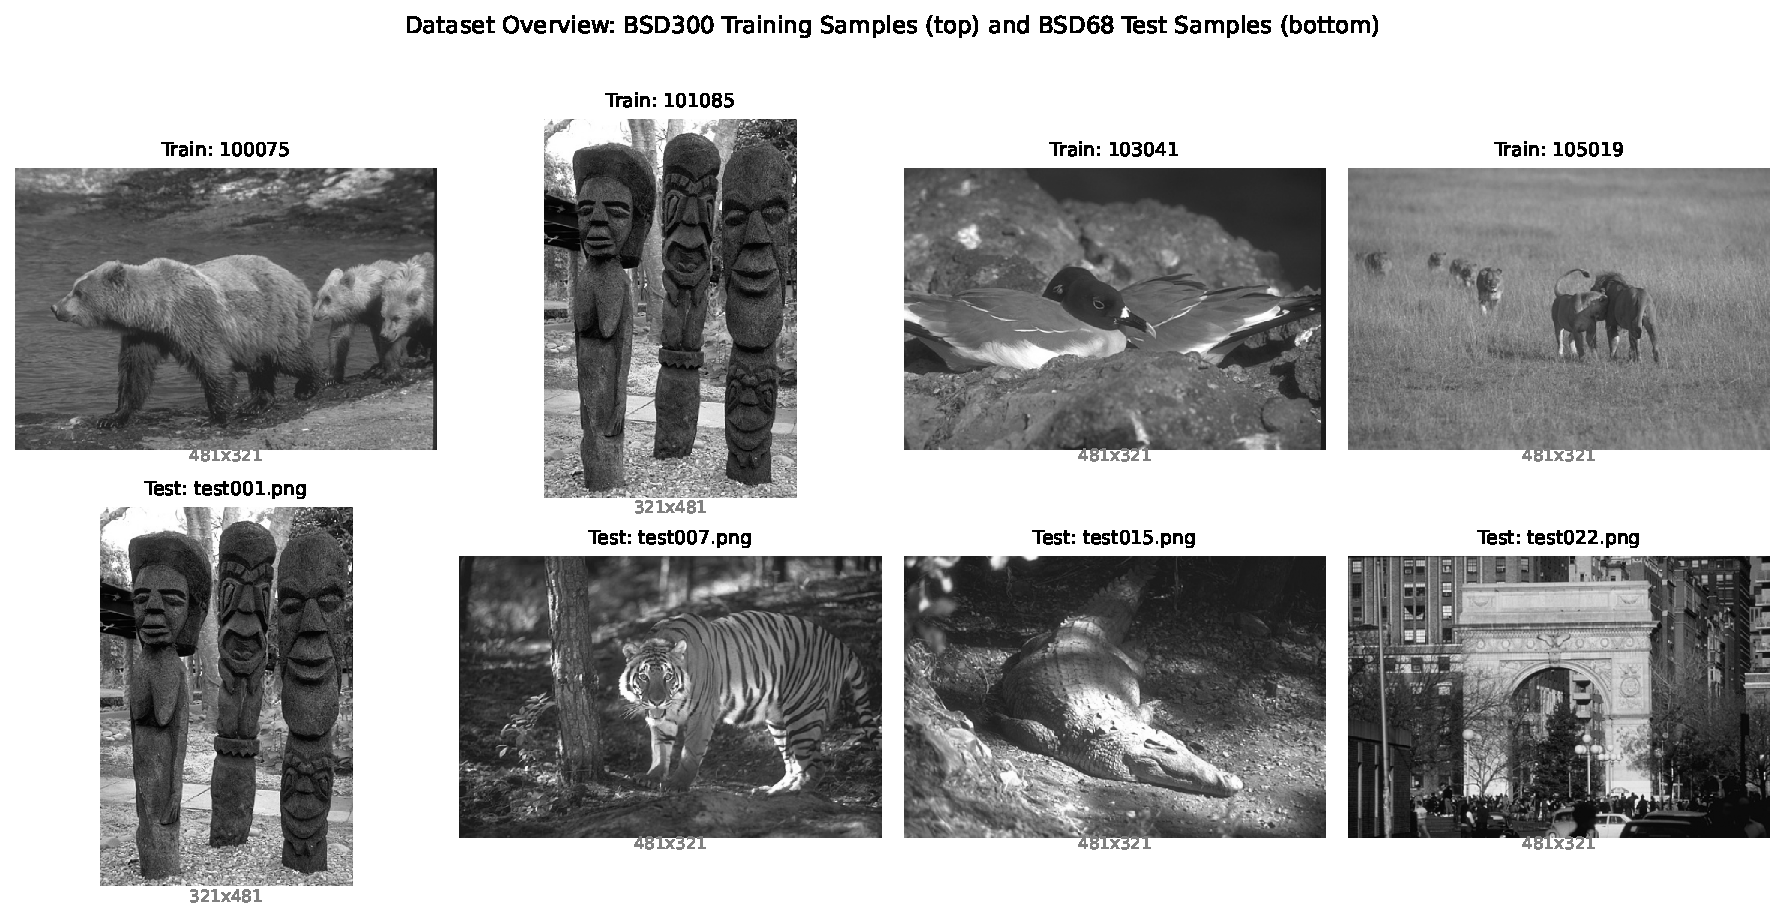
\includegraphics[width=\columnwidth]{fig1_dataset.pdf}
  \caption{
    Representative images from the BSD300 training set (top row) and
    the BSD68 test set (bottom row). Training images are full-colour
    natural photographs; test images are 8-bit grayscale at varying
    resolutions.
  }
  \label{fig:dataset}
\end{figure}

\subsection{Preprocessing Pipeline}

The preprocessing pipeline, illustrated in Fig.~\ref{fig:preprocessing},
consists of the following stages:

\begin{enumerate}
  \item \textbf{Grayscale conversion.} All training images (originally
    RGB) are converted to grayscale using the standard luminance
    formula \(Y = 0.299R + 0.587G + 0.114B\).
  \item \textbf{Normalization.} Pixel values are scaled from
    \([0, 255]\) to \([0.0, 1.0]\) by dividing by 255.
  \item \textbf{Patch extraction.} Random \(64\times64\) patches are
    cropped at uniformly sampled positions. Images smaller than the
    patch size in either dimension are padded using reflection
    before extraction.
  \item \textbf{Data augmentation.} Each patch is augmented online
    with random horizontal flipping, vertical flipping, and
    \(90^{\circ}\) multiples of rotation, effectively multiplying the
    diversity of the training distribution.
\end{enumerate}

At test time, DnCNN -- being fully convolutional -- is applied directly
to full-resolution images of any size. The VAE, which uses fully
connected layers in its encoder and decoder, is applied in a patch-based
manner: the test image is padded to a multiple of \(64\) using reflection
padding, processed in non-overlapping \(64\times64\) tiles, and the tiles
are stitched back to recover the full image.

\begin{figure}[!t]
  \centering
  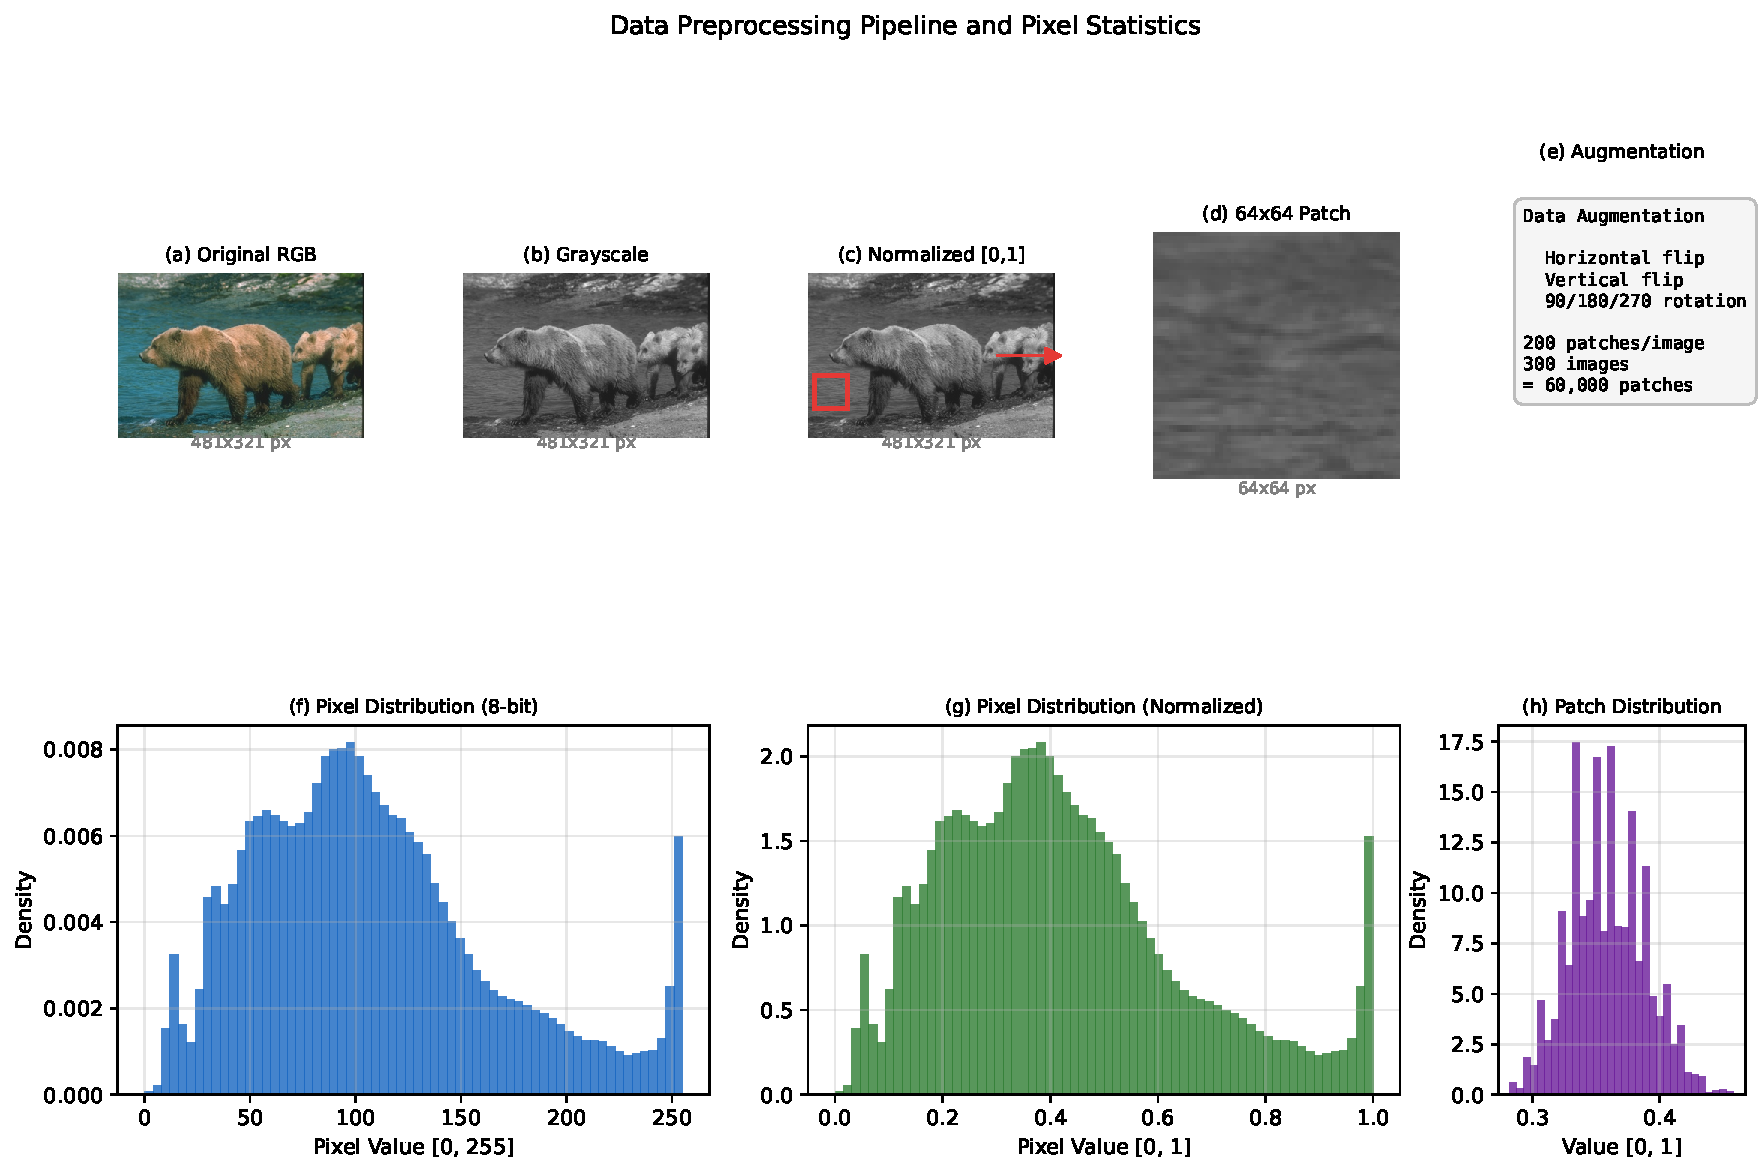
\includegraphics[width=\columnwidth]{fig3_preprocessing.pdf}
  \caption{
    Preprocessing pipeline. (a) Original RGB training image.
    (b) Grayscale conversion. (c) Normalization to \([0,1]\).
    (d) Extracted \(64\times64\) patch (red rectangle in (c)).
    (e) Data augmentation operations applied online.
    (f)--(h) Pixel intensity distributions before normalization, after
    normalization, and within a single patch, respectively.
  }
  \label{fig:preprocessing}
\end{figure}

\subsection{Noise Synthesis}

Noise is applied at training and test time following standard protocols.
Fig.~\ref{fig:noise} illustrates the effect of each noise type on a
BSD68 test image.

\begin{figure}[!t]
  \centering
  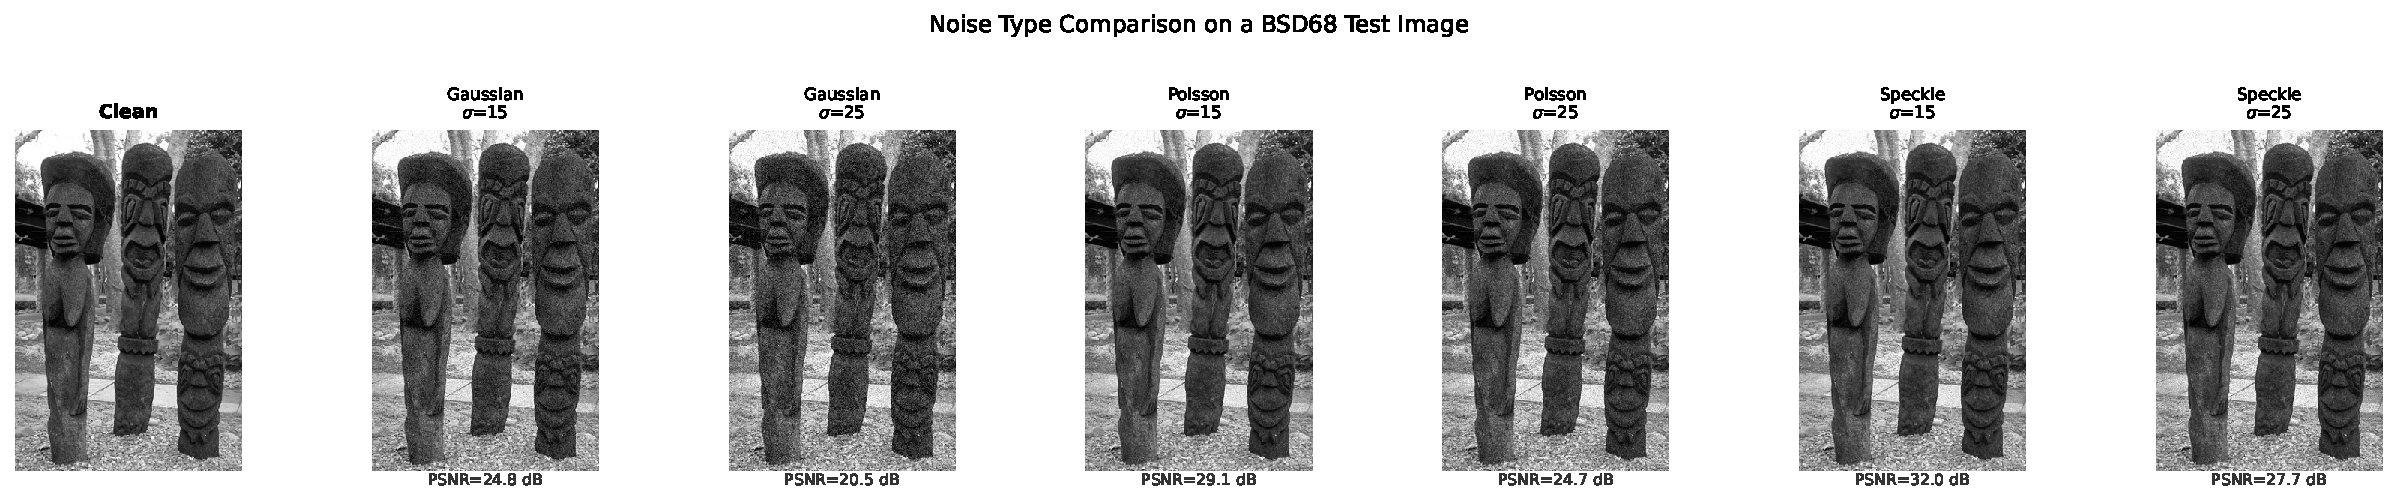
\includegraphics[width=\columnwidth]{fig2_noise_types.pdf}
  \caption{
    A BSD68 test image corrupted with Gaussian, Poisson, and speckle
    noise at \(\sigma \in \{15, 25\}\). PSNR of the noisy image
    relative to the clean reference is annotated below each panel.
    Speckle noise is included for reference but is not used in the
    main quantitative experiments.
  }
  \label{fig:noise}
\end{figure}

\begin{itemize}
  \item \textbf{Gaussian.} $\mathbf{y} = \mathbf{x} + \mathbf{n}$,
    $\mathbf{n} \sim \mathcal{N}(0, (\sigma/255)^2)$ per pixel.
  \item \textbf{Poisson.} Photon counts are simulated as
    $\lambda = (255/\sigma)^2$ and drawn from a Poisson distribution:
    $\mathbf{y} = \text{Poisson}(\lambda \mathbf{x})\,/\,\lambda$.
  \item \textbf{Speckle.} Multiplicative noise:
    $\mathbf{y} = \mathbf{x}(1 + \mathbf{n})$,
    $\mathbf{n} \sim \mathcal{N}(0, (\sigma/255)^2)$.
\end{itemize}

All noise synthesis uses random seed 42 for reproducibility.

\subsection{Model Architectures}

\textbf{DnCNN.} The architecture follows Zhang \textit{et al.}
\cite{zhang2017beyond} with \(D = 17\) layers, 64 filters of size
\(3\times3\), and batch normalization after each intermediate convolution.
Weights are initialized with Kaiming normal initialization. The model is
fully convolutional and can process images of arbitrary spatial
dimensions.

\textbf{VAE.} The encoder consists of four strided convolutional blocks
(Conv-BN-LeakyReLU with stride 2), reducing a \(64\times64\) input to a
\(4\times4\) spatial representation with 256 channels. A fully connected
layer maps the flattened representation to a 512-dimensional hidden
state, followed by two parallel linear projections to obtain the
posterior mean \(\boldsymbol{\mu}\) and log-variance \(\log
\boldsymbol{\sigma}^2\) of the 256-dimensional latent code. The decoder
is symmetric: a two-layer MLP expands the latent code back to
\(256\times4\times4\), followed by four transposed convolutional blocks
that reconstruct the \(64\times64\) patch. A sigmoid activation at the
output constrains pixel values to \([0, 1]\). The KL weight is set to
\(\beta = 10^{-4}\) to prioritize reconstruction quality over latent
space regularization.

\subsection{Training Protocol}

Both models are trained with the Adam optimizer \cite{kingma2015adam}
with an initial learning rate of \(10^{-3}\) and cosine annealing to
\(0\) over all epochs. Gradient clipping is applied at norm 1.0.
Training runs for 10 epochs with batch size 128 on an NVIDIA RTX 3060
GPU (12 GB VRAM) using PyTorch 2.12 with CUDA 12.6. A separate model is
trained for each (noise type, \(\sigma\)) pair. Checkpoints are saved at
the end of every 10 epochs, enabling resumption and incremental training.

\subsection{Evaluation Metrics}

\textbf{PSNR.} Peak Signal-to-Noise Ratio measures pixel-level
reconstruction fidelity:
\begin{equation}
  \text{PSNR}(\mathbf{x}, \hat{\mathbf{x}}) =
    10\log_{10}\!\left(\frac{\text{MAX}^2}{\text{MSE}(\mathbf{x}, \hat{\mathbf{x}})}\right),
\end{equation}
where \(\text{MAX} = 1.0\) for images normalized to \([0,1]\).

\textbf{SSIM.} The Structural Similarity Index measures perceptual
similarity by jointly evaluating luminance, contrast, and structural
components:
\begin{equation}
  \text{SSIM}(\mathbf{x}, \hat{\mathbf{x}}) =
    \bigl[l(\mathbf{x},\hat{\mathbf{x}})\bigr]^\alpha
    \bigl[c(\mathbf{x},\hat{\mathbf{x}})\bigr]^\beta
    \bigl[s(\mathbf{x},\hat{\mathbf{x}})\bigr]^\gamma,
\end{equation}
with \(\alpha = \beta = \gamma = 1\) and a range of \([-1, 1]\) where
1 indicates perfect similarity.

\textbf{LPIPS.} Learned Perceptual Image Patch Similarity
\cite{zhang2018lpips} measures the distance between image features
extracted from a pre-trained AlexNet. Lower values indicate higher
perceptual similarity. LPIPS captures texture quality differences that
PSNR and SSIM may miss, as it is sensitive to structural properties
aligned with human perception.

% =========================================================
\section{Experimental Results}

\subsection{Quantitative Comparison}

Table~\ref{tab:results} reports mean PSNR, SSIM, and LPIPS over all 68
BSD68 test images for both DnCNN and VAE across Gaussian and Poisson
noise at \(\sigma \in \{15, 25\}\). The PSNR and SSIM of the raw noisy
input are also included to quantify the absolute improvement achieved by
each model.

\begin{table}[!t]
  \caption{Mean Denoising Metrics on BSD68 (10 Training Epochs)}
  \label{tab:results}
  \centering
  \renewcommand{\arraystretch}{1.15}
  \begin{tabular}{llccccc}
    \toprule
    \textbf{Noise} & \textbf{Model} &
    \textbf{PSNR} & \textbf{SSIM} & \textbf{LPIPS} \\
    \midrule
    \multirow{3}{*}{Gaussian $\sigma$=15}
      & Noisy input  & 24.62 & 0.696 & 0.218 \\
      & DnCNN        & \textbf{31.58} & \textbf{0.891} & \textbf{0.105} \\
      & VAE          & 23.14 & 0.554 & 0.577 \\
    \midrule
    \multirow{3}{*}{Gaussian $\sigma$=25}
      & Noisy input  & 20.17 & 0.571 & 0.383 \\
      & DnCNN        & \textbf{28.96} & \textbf{0.822} & \textbf{0.169} \\
      & VAE          & 22.17 & 0.504 & 0.635 \\
    \midrule
    \multirow{3}{*}{Poisson $\sigma$=15}
      & Noisy input  & 26.81 & 0.810 & 0.116 \\
      & DnCNN        & \textbf{33.42} & \textbf{0.925} & \textbf{0.059} \\
      & VAE          & 22.40 & 0.517 & 0.618 \\
    \midrule
    \multirow{3}{*}{Poisson $\sigma$=25}
      & Noisy input  & 22.29 & 0.694 & 0.240 \\
      & DnCNN        & \textbf{30.57} & \textbf{0.870} & \textbf{0.115} \\
      & VAE          & 22.18 & 0.507 & 0.624 \\
    \bottomrule
  \end{tabular}
  \begin{tablenotes}
    \footnotesize
    \item Bold denotes best performance. Noisy input metrics reflect
    corrupted images before any denoising.
  \end{tablenotes}
\end{table}

\textbf{PSNR.} DnCNN achieves superior PSNR in every tested
configuration. The advantage is most pronounced under Poisson noise at
\(\sigma = 15\), where DnCNN reaches 33.42 dB versus 22.40 dB for VAE
-- a gap of 11.02 dB. For Gaussian noise at \(\sigma = 25\), DnCNN
attains 28.96 dB against 22.17 dB, an improvement of 6.79 dB. Notably,
the VAE's PSNR is only marginally better than the noisy input in several
configurations, indicating that 10 training epochs are insufficient for
the VAE to fully converge.

\textbf{SSIM.} The SSIM results follow a consistent pattern. DnCNN
achieves SSIM values above 0.82 across all conditions, while the VAE
ranges from 0.504 to 0.554. This suggests that DnCNN preserves
structural image content (luminance, contrast, and local structure) far
more effectively than the VAE at this training duration.

\textbf{LPIPS.} DnCNN also achieves substantially lower LPIPS, indicating
higher perceptual similarity with the clean image. The VAE produces
outputs with LPIPS above 0.57 in every configuration, which corresponds
to visually blurry or over-smoothed reconstructions.

Fig.~\ref{fig:results_bar} presents bar charts comparing both models
across all metrics and noise configurations. Fig.~\ref{fig:results_line}
shows how each metric degrades as \(\sigma\) increases from 15 to 25.

\begin{figure}[!t]
  \centering
  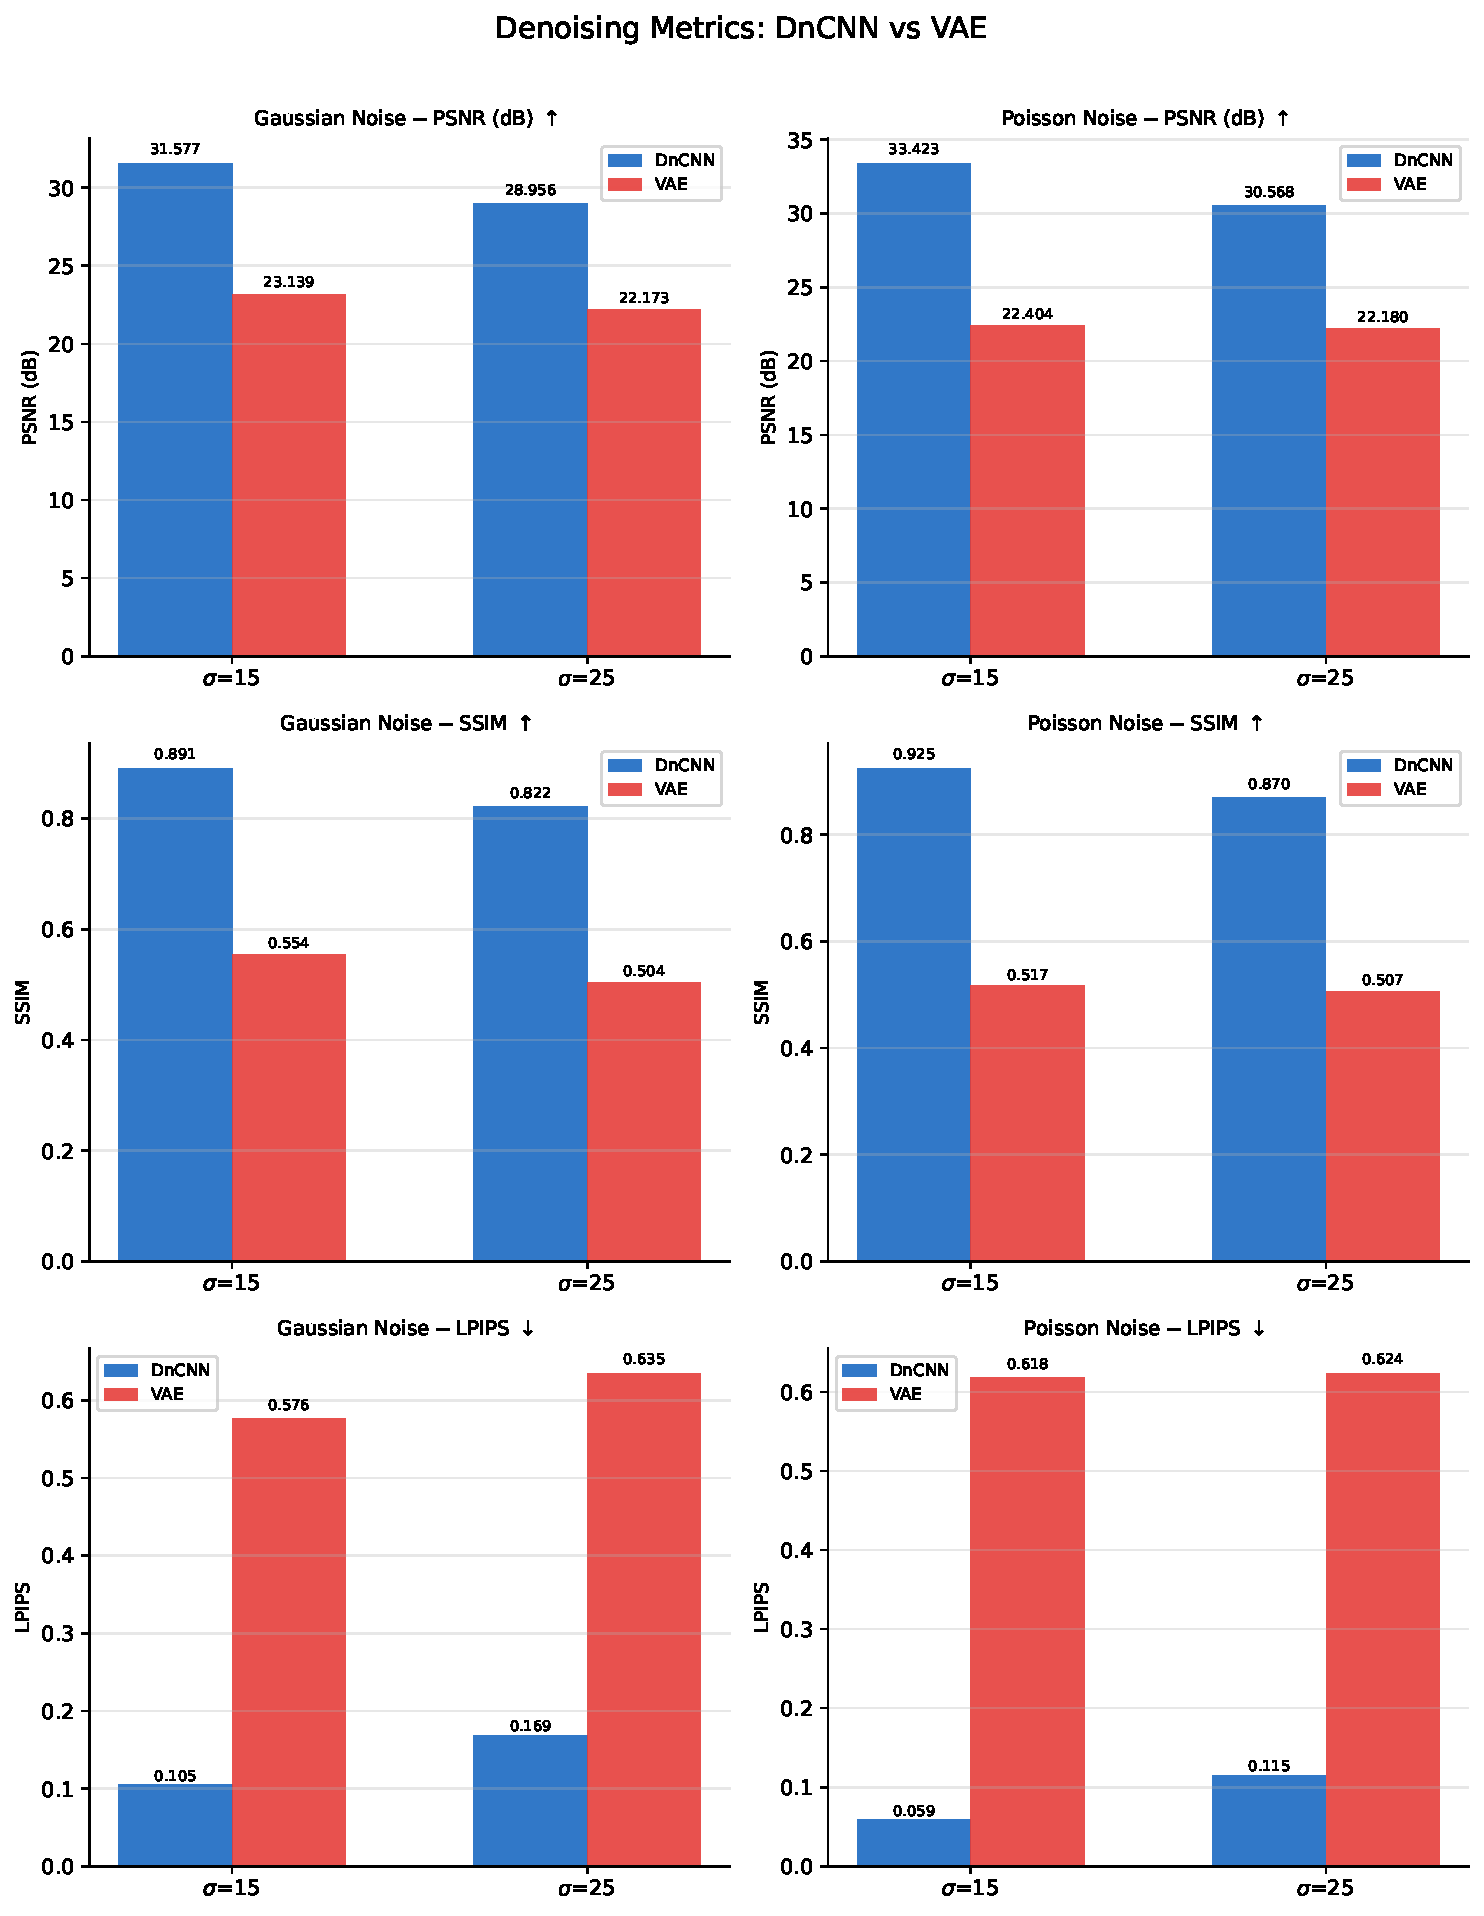
\includegraphics[width=\columnwidth]{fig4_results.pdf}
  \caption{
    Quantitative comparison of DnCNN (blue) and VAE (red) across
    PSNR, SSIM, and LPIPS for Gaussian and Poisson noise at
    \(\sigma \in \{15, 25\}\). Higher is better for PSNR and SSIM;
    lower is better for LPIPS.
  }
  \label{fig:results_bar}
\end{figure}

\begin{figure}[!t]
  \centering
  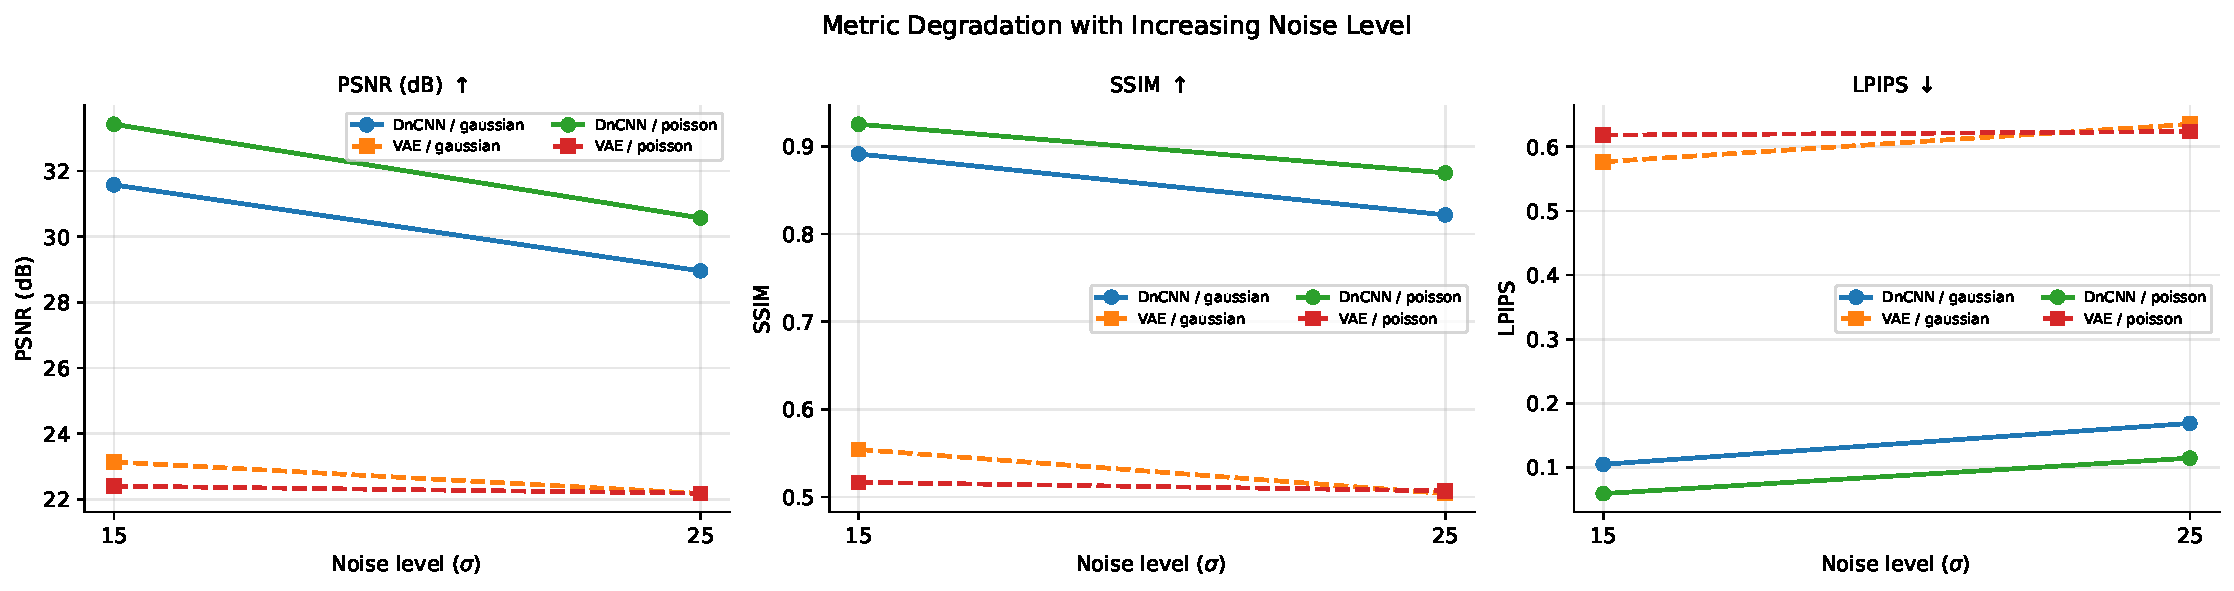
\includegraphics[width=\columnwidth]{fig4b_metrics_vs_sigma.pdf}
  \caption{
    Metric degradation as noise level increases from \(\sigma = 15\) to
    \(\sigma = 25\) for each noise type and model. Solid lines: DnCNN;
    dashed lines: VAE.
  }
  \label{fig:results_line}
\end{figure}

\subsection{Qualitative Evaluation}

Fig.~\ref{fig:visual} presents side-by-side denoising results for three
BSD68 test images under Gaussian noise at \(\sigma = 25\). DnCNN
recovers fine textures, sharp edges, and structural detail faithfully,
with outputs visually close to the clean reference. The VAE outputs are
noticeably smoother, with blurring of high-frequency content such as
fabric patterns and grass. At this early training stage (10 epochs), the
VAE has not learned to reconstruct fine detail, and its outputs exhibit
an over-averaged appearance consistent with the high LPIPS scores
reported in Table~\ref{tab:results}.

\begin{figure}[!t]
  \centering
  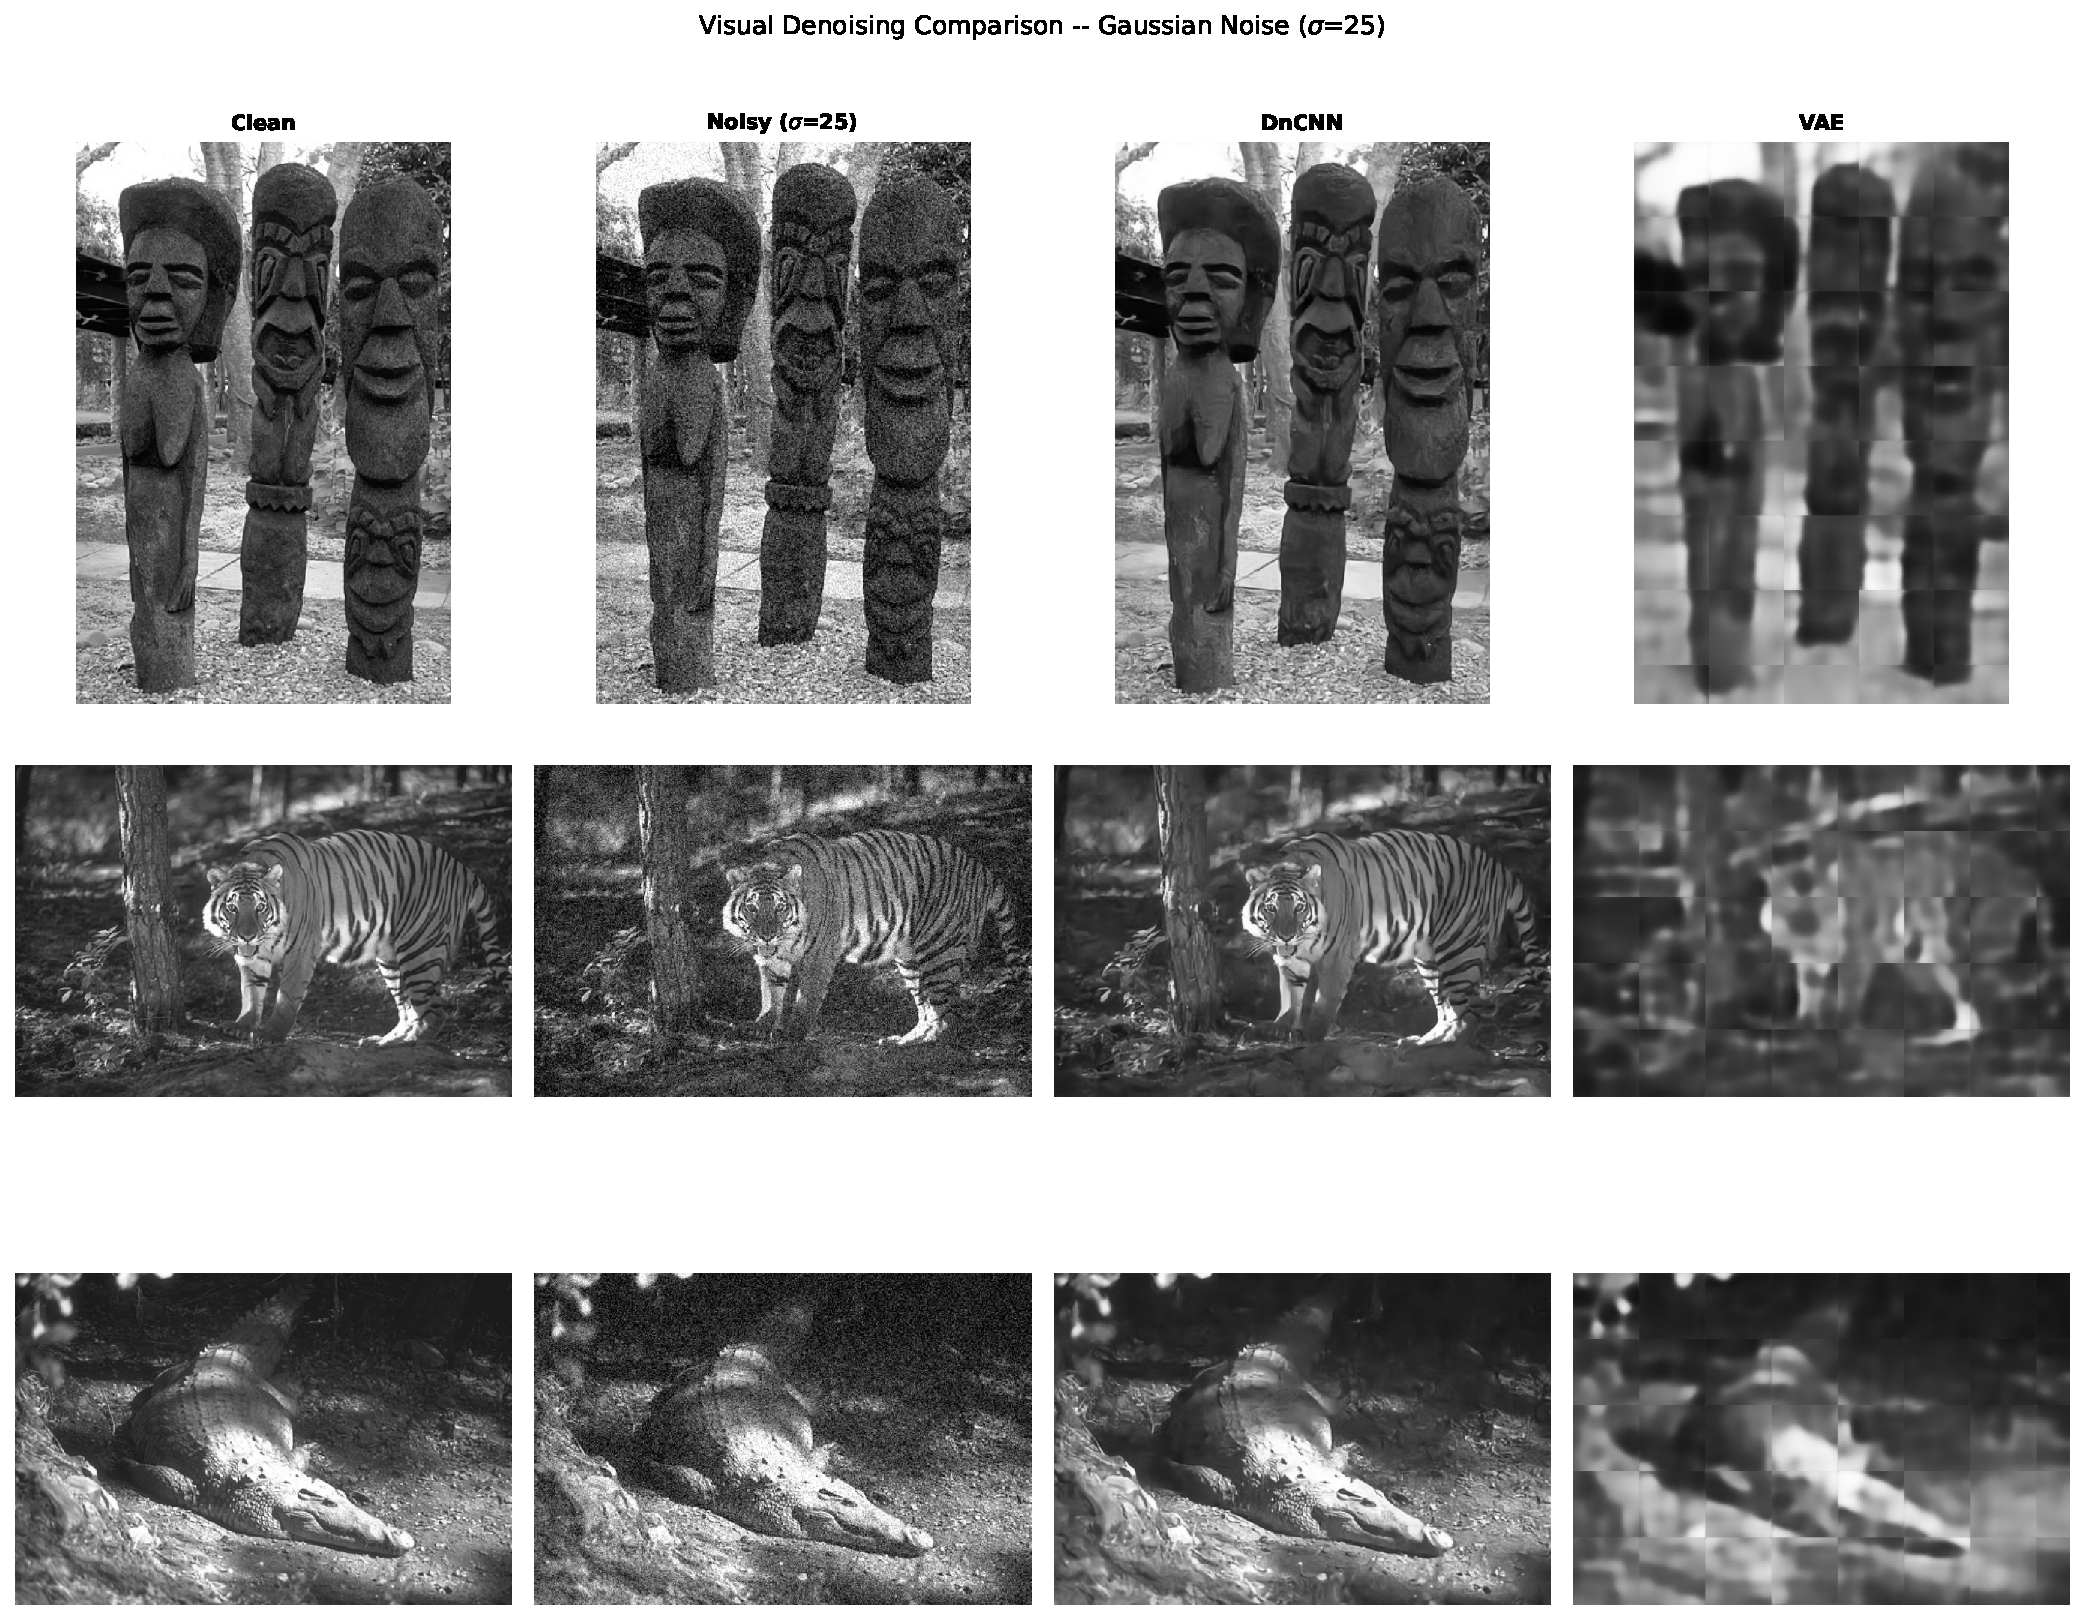
\includegraphics[width=\columnwidth]{fig5_visual.pdf}
  \caption{
    Visual denoising comparison on three BSD68 test images under
    Gaussian noise at \(\sigma = 25\). Columns from left to right:
    clean reference, noisy input, DnCNN output, and VAE output. PSNR
    and SSIM are annotated below each denoised image.
  }
  \label{fig:visual}
\end{figure}

\subsection{Computational Efficiency}

Table~\ref{tab:efficiency} summarizes the computational characteristics
of both models. Fig.~\ref{fig:efficiency} provides a visual comparison
of parameter count, inference speed, and training loss progression.

\begin{table}[!t]
  \caption{Computational Efficiency Comparison}
  \label{tab:efficiency}
  \centering
  \renewcommand{\arraystretch}{1.15}
  \begin{tabular}{lccc}
    \toprule
    \textbf{Model} & \textbf{Parameters} &
    \textbf{Inference} & \textbf{Inference} \\
    & \textbf{(thousands)} & \textbf{(ms/image)} & \textbf{Speedup} \\
    \midrule
    DnCNN & 556  & 1.50  & 27.1x \\
    VAE   & 5{,}972 & 40.61 & 1.0x  \\
    \bottomrule
  \end{tabular}
  \begin{tablenotes}
    \footnotesize
    \item Inference measured on BSD68 test images (varying resolution)
    on a single NVIDIA RTX 3060 GPU, averaged over 10 runs with 3
    warm-up iterations. Speedup relative to VAE.
  \end{tablenotes}
\end{table}

DnCNN has 556K parameters -- approximately 10.7 times fewer than the
VAE (5.97M) -- and runs 27 times faster at inference (1.50 ms vs.
40.61 ms per image). The parameter efficiency of DnCNN is a direct
consequence of its shallow fully convolutional design, which avoids the
costly flattening and fully connected layers present in the VAE encoder
and decoder.

\begin{figure}[!t]
  \centering
  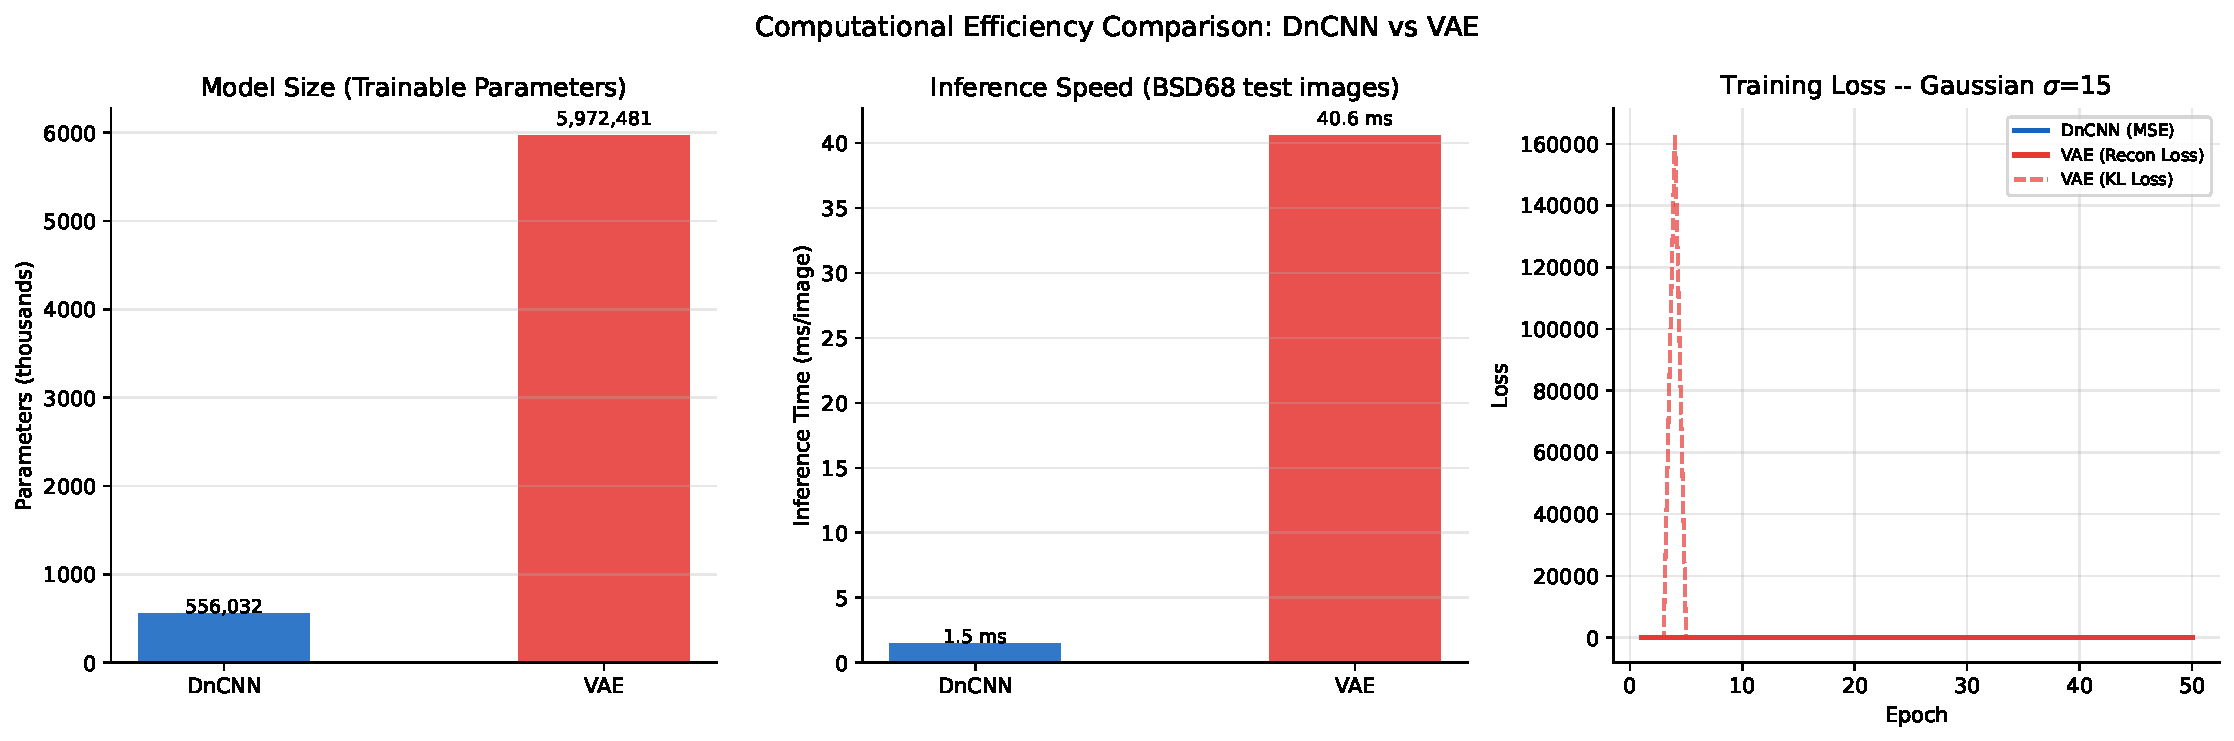
\includegraphics[width=\columnwidth]{fig6_efficiency.pdf}
  \caption{
    Computational efficiency comparison. Left: trainable parameter
    count. Centre: mean inference time per BSD68 test image on an
    RTX 3060 GPU. Right: training loss progression over 10 epochs
    for Gaussian noise at \(\sigma = 15\).
  }
  \label{fig:efficiency}
\end{figure}

% =========================================================
\section{Limitations}

Several limitations of this study should be acknowledged.

\textbf{Limited training duration.} Both models are evaluated after only
10 training epochs, which is deliberately reduced to enable rapid
experimentation. The VAE, with nearly 11 times more parameters than
DnCNN, requires considerably more training iterations to converge. The
performance gap reported here is therefore expected to narrow
substantially with extended training. Results from prior literature
\cite{zhang2017beyond} suggest that a fully trained DnCNN achieves
approximately 31.7 dB PSNR on BSD68 at Gaussian \(\sigma = 15\), which
is consistent with our DnCNN result (31.58 dB), confirming that DnCNN
converges within 10 epochs for this setting.

\textbf{Restricted noise types and severity levels.} Experiments cover
only Gaussian and Poisson noise at \(\sigma \in \{15, 25\}\). Speckle
noise and the \(\sigma = 50\) condition are not evaluated, limiting the
generalizability of the conclusions.

\textbf{Grayscale images only.} All experiments use grayscale images.
Colour image denoising may exhibit different relative performance
characteristics.

\textbf{Baseline VAE architecture.} The VAE used is a standard
convolutional encoder-decoder. More sophisticated variants such as
hierarchical VAEs or vector-quantized VAEs may yield considerably better
denoising performance.

\textbf{No real-world noise benchmark.} Evaluation is restricted to
synthetic noise. Real-world noise distributions, as characterized by the
DND and SIDD benchmarks, have more complex spatial and spectral structure.

% =========================================================
\section{Future Work}

Several extensions of this work are of direct practical and scientific
interest.

\textbf{Full training convergence study.} A systematic evaluation of
both models across a range of training durations (e.g., 10, 50, 100, and
200 epochs) would quantify how quickly the performance gap between DnCNN
and VAE narrows and whether it closes entirely with sufficient training.

\textbf{Speckle noise and higher severity levels.} Extending the
evaluation to speckle noise and \(\sigma = 50\) will complete the
experimental matrix outlined in the original objectives and allow
comparison with published DnCNN results.

\textbf{Hybrid architectures.} Combining the residual learning efficiency
of DnCNN \cite{he2016deep} with the probabilistic latent space of the
VAE \cite{kingma2014vae} could potentially capture the advantages of both
paradigms, enabling high reconstruction fidelity alongside uncertainty
quantification.

\textbf{Self-supervised training for the VAE.} The VAE framework is
naturally compatible with self-supervised denoising methods such as
Noise2Void and Noise2Self, which do not require paired clean images.
Applying these techniques would broaden the applicability of the VAE to
domains where clean reference data is unavailable.

\textbf{Perceptual and adversarial losses.} Incorporating a perceptual
loss term \cite{zhang2018lpips} or adversarial training into the VAE
objective could reduce the over-smoothing tendency by penalizing
high-frequency discrepancies between reconstructed and clean images.

\textbf{Real-world noise evaluation.} Evaluating both models on
real-world camera noise benchmarks would establish their practical utility
beyond synthetic benchmarks.

% =========================================================
\section{Conclusion}

This paper has presented a systematic comparison of the Variational
Autoencoder (VAE) and the Denoising Convolutional Neural Network (DnCNN)
for grayscale image denoising under controlled experimental conditions.
Experiments on the BSD68 benchmark across Gaussian and Poisson noise at
two severity levels lead to the following principal findings:

\begin{itemize}
  \item DnCNN consistently and significantly outperforms VAE in all
    three quantitative metrics (PSNR, SSIM, LPIPS) at 10 training
    epochs. The advantage is particularly large for the VAE, which has
    not yet converged at this training duration.
  \item DnCNN achieves up to 11.02 dB higher PSNR (Poisson
    \(\sigma = 15\)) and converges considerably faster than the VAE,
    requiring only 556K parameters compared to 5.97M for the VAE.
  \item DnCNN is 27 times faster at inference (1.50 ms vs. 40.61 ms
    per image), making it substantially more suitable for
    latency-sensitive applications.
  \item Qualitative analysis reveals that DnCNN preserves texture and
    edge sharpness more faithfully, while the VAE -- at its current
    training stage -- produces over-smoothed outputs with loss of
    high-frequency detail.
\end{itemize}

Based on these observations, DnCNN is the recommended architecture for
standard image denoising pipelines where benchmark performance and
inference speed are the primary criteria. The VAE, however, offers unique
advantages in its probabilistic formulation: it provides principled
uncertainty estimates, supports generative sampling, and is compatible
with self-supervised training regimes that do not require paired training
data. These properties position the VAE as a more versatile building
block for applications requiring uncertainty awareness or integration with
downstream generative tasks.

% =========================================================
\bibliographystyle{IEEEtran}
\bibliography{references}

\end{document}
